\section{The functional reference architecture of the perception chain}\label{sec:refarchitecture}
This section develops a functional reference architecture for the perception chain allowing to provably bound the risk for misperceptions. The following principles guided this proposal:
\begin{enumerate}
\item It must be possible to bound the contributions to risks for each component of the perception chain.
\item This entails the need to specify for each element in the perception conditions under which this element can be \enquote{trusted}. Violations of such conditions must be monitored and -- if persistent -- must induce declaration of \enquote{blindness}, automatically inducing minimal risk maneuvers.\todo{Ist das "blame principle" von MobilEye ein Minimum Risk Maneuver? Es erlaubt eine wuenschenswerte Art von Blindness...}
\item The reference architecture must provide guidance as to the degree of precision of perception required for current maneuver decisions.
\end{enumerate}
We discuss the implications of these design principles in separate subsections, along the flow through the perception chain.

\subsection{Quality criteria for sensor components}\label{subsec:quality}

While radar systems are widely deployed for variants of ACC systems and emergency breaking systems, their integration in level 3, 4, or 5 HAVs constitutes a completely different operational context, because the overall safety case can no longer rely on human supervision of the environment of the ego car. Well known phenomena such as ghost objects stemming from undesired and uncontrollable reflections, or \enquote{stealth type cars} such as the VW beetle, or simply reflections induced by metal-coating of truck planes are but examples of a plethora of phenomena, which all influence quality of object detection through radar. With the transition to level 3, 4, 5 systems, quality criteria must take a more rigid form: we must be able to quantify the risks of missing objects, or showing ghost objects. Similar types of distortion of perception are well known and documented for Lidar systems in certain types of rain conditions, for video systems in certain types of lighting conditions, etc. We propose a uniform quality measure for different type of sensor systems, by assessing their capability to contribute to detecting all relevant objects in the what is often called the occupancy grid enclosing the ego car. Specifically, we take a suitable 3d extension of the electronic horizon of the ego vehicle, and assume a sufficiently fine grained, not necessarily homogeneous partitioning of this 3d space, and refer to this as \emph{occupancy grid(ego)}. We view sensors as providing labels of the partitions of the occupancy grid, providing information about whether a given sensor has identified some artifact in this grid partition, depending on sensor type filled with additional information such as speed (for radar), temperature (for infrared), gray-scale distribution of pixels for video cameras, \ldots, typically as distributions with confidence levels, e.g. regarding the likelihood of some artifact being located in this grid partition. The formal quality requirement is just an instantiation of the safe perception requirement in formula (1). Specifically, for a given position \textit{pos}  of sensor  \textit{s}  on vehicle ego, let us denote by \textit{visible(s,pos)} the coherent subspace of the occupancy grid covered by sensor \textit{s} when mounted at this position, then for any relevant artifact  $a$, and any property  \textit{label($a$)} discernable by  \textit{s}  in this position, we would want the sensor \textit{s} to almost always, up to some bounded risk $r_s$, correctly label the grid field with \textit{label($a$)} at time $t$, when $a$ is at a visible grid partition in ground truth, as determined by the state of \textit{TS(ego)} at that point in time:

\begin{align}\label{eq:safelabelling(s,pos)}
    \textit{Safe}\_&\textit{labelling(s,pos)} \equiv 					\\		
 & \forall a\in\textit{ observables(TS(ego))}\forall p \in \textit{occupancy grid(ego)}:\nonumber\\  
& \Box (\textit{relevant}(a) \land a \textit{ is at } p\land p\in \textit{visible(s,pos)} \nonumber\\
& \Rightarrow P(\neg( \Box_{\leq\Delta} d_{a,s}(a,\textit{label}(a))\leq\delta_{a,s}))) < r_s\nonumber
\end{align}

Since phenomena such as reflections discussed above will have strong negative impact on achieving sufficiently precise distances between beliefs and ground truth, we propose to characterize for each sensor adverse conditions. Only by separating out such conditions can we obtain a sufficiently tight bound on the risks of incorrect labelling of the occupancy grid, to achieve an overall risk tolerated by society. The down side is the need to then also identify reliably such adverse conditions; in this paper, we integrate such adverse conditions in our ontology, and then use the full power of the perception chain to learn sufficiently reliable classifications of adverse conditions, see next subsection. As in \cite{galbas}, we propose to use learning techniques from field observations to characterize adverse conditions for each sensor \textit{s} and to derive such quality guarantees. We now weaken formula (2) by weakening the criteria for sufficient precision of beliefs in that no promises regarding precision are made when adverse conditions $ad$ occur:

\begin{align}\label{eq:safelabelling(s,pos,ad)}
\textit{Safe}\_&\textit{labelling(s,pos,ad)} \equiv\\  			
&\forall a\in \textit{observables(TS(ego))}\forall p\in\textit{occupancy grid(ego)}\nonumber:\\
&\Box(\textit{relevant(a)} \land a\textit{ is at p }\land p\in\textit{visible(s,pos)} \Rightarrow\nonumber\\
&P(\neg(\Box_{\leq\Delta} (d_{a,s}(a, \textit{label(a)})\leq \delta_{a,s}))\textit{ unless } ad)) < r_s\nonumber
\end{align}

Note that we can in particular encode the constraints of a given ODD in such adverse conditions, which thus entails that information of a sensor is not trusted if working outside the constraints of the ODD. OEMs compensate weaknesses of types of sensor systems by providing redundancy and diversity and using sensor fusion. We can derive a composed sensor s from fusing two qualified positioned sensors $<$s1,pos1$>$  and $<$s2,pos2$>$ to system s as follows:
\begin{itemize}
\item ad(s) is the disjunction of ad(s1) and ad(s2)
\item visible(s) = visible($<$s1,pos1$>$) $\cup$ visible($<$s2,pos2$>$)
\item for each $p\in $\textit{occupancy grid(ego)}:  \\
if p $\in$ visible($<$s1,pos1$>$) $\cap$ visible($<$s2,pos2$>$) then
\begin{itemize}
\item if $\neg$ad(s1)$\land\neg$ ad(s2) then\\
if label(s1)(p) $\land$ label(s2)(p) $\not=$ false 
\begin{itemize}
\item[] then label(s)(p) := label(s1)(p) $\land $label(s2)(p)
\item[] else label(s)(p) := $\bot$
\end{itemize}\todo{Weiss nicht wie man es besser machen soll, aber die Nichtmonotonie, dass man hier im besser informierten Fall pessimistischere Label zuordnet als wenn ein Sensor erblindet ist, stoesst mir auf.}
\todo[inline]{WH: das letzte if--then--else l\"asst sich zu "label(s)(p) := label(s1)(p) $\land$ label(s2)(p)" zusammenfassen (da $\bot$ ja gerade false repr\"asentiert).}
\item[] else if ad(s1)$\land\neg$ad(s2) then label(s)(p) := label(s1)
\item[] else if $\neg$ad(s1)$\land$ad(s2) then label(s)(p) := label(s2)
\item[] else if ad(s1) $\land$ ad(s2) then label(s) := $\bot$
\end{itemize}
\item[] else if p$\in$visible($<$s1,pos1$>$) $\setminus$ visible($<$s2,pos2$>$) then\\	
if $\neg$ad(s1)
\begin{itemize}
    \item[] then label(s) := label(s1)
	\item[] else if ad(s1) then label(s) := $\bot$
	\end{itemize}
	else if p $\in$ visible($<$s2,pos2$>$) $\setminus$ visible($<$s1,pos1$>$) then
	\begin{itemize}
	\item[] if $\neg$ad(s2) 
	\begin{itemize}
	    \item[]then label(s) := label(s2)
	\item[] else if ad(s2) then label(s) := $\bot$
    \end{itemize}
    \end{itemize}
\end{itemize}
Note that any detected inconsistencies are marked $\bot$. Also the combined sensor labels fields p with $\bot$ if p is only visible for one sensor, but this sensor cannot be trusted because of prevailing adverse conditions. We derive quality guarantees for sensor fusion in Section \ref{sec:proofrule}. For observations where both sensors are in non-adverse conditions, and both sensors observe p, then the risk of misclassifications is reduced to $r_{s1} \times r_{s2}$ if we can prove that misperceptions are stochastically independent under operating conditions favorable for both sensors, otherwise the risks for misperception of the fused systems for fields p visible to both sensors is min($r_{s1}$,$r_{s2}$).

Level 4 and 5 HAVs must guarantee by construction sensor completeness with maximal risk r: for all points in time, and all relevant fields p of the occupancy grid, there must at least be one positioned sensor operating in non-adverse conditions, such that p is visible for this sensor, and the risk of misperception by this sensor is smaller than r, unless there are multiple positioned sensors all operating in non-adverse conditions, which are stochastically independent under such conditions; in this case the products of their risk levels must be smaller than r. Since this property is more easily expressed using the formula derived in Section \ref{sec:proofrule} for sensor fusion, we formalize this key requirement of sensor completeness in Section \ref{sec:proofrule}.

\subsection{The functional reference architecture}

\begin{figure}
    \centering
    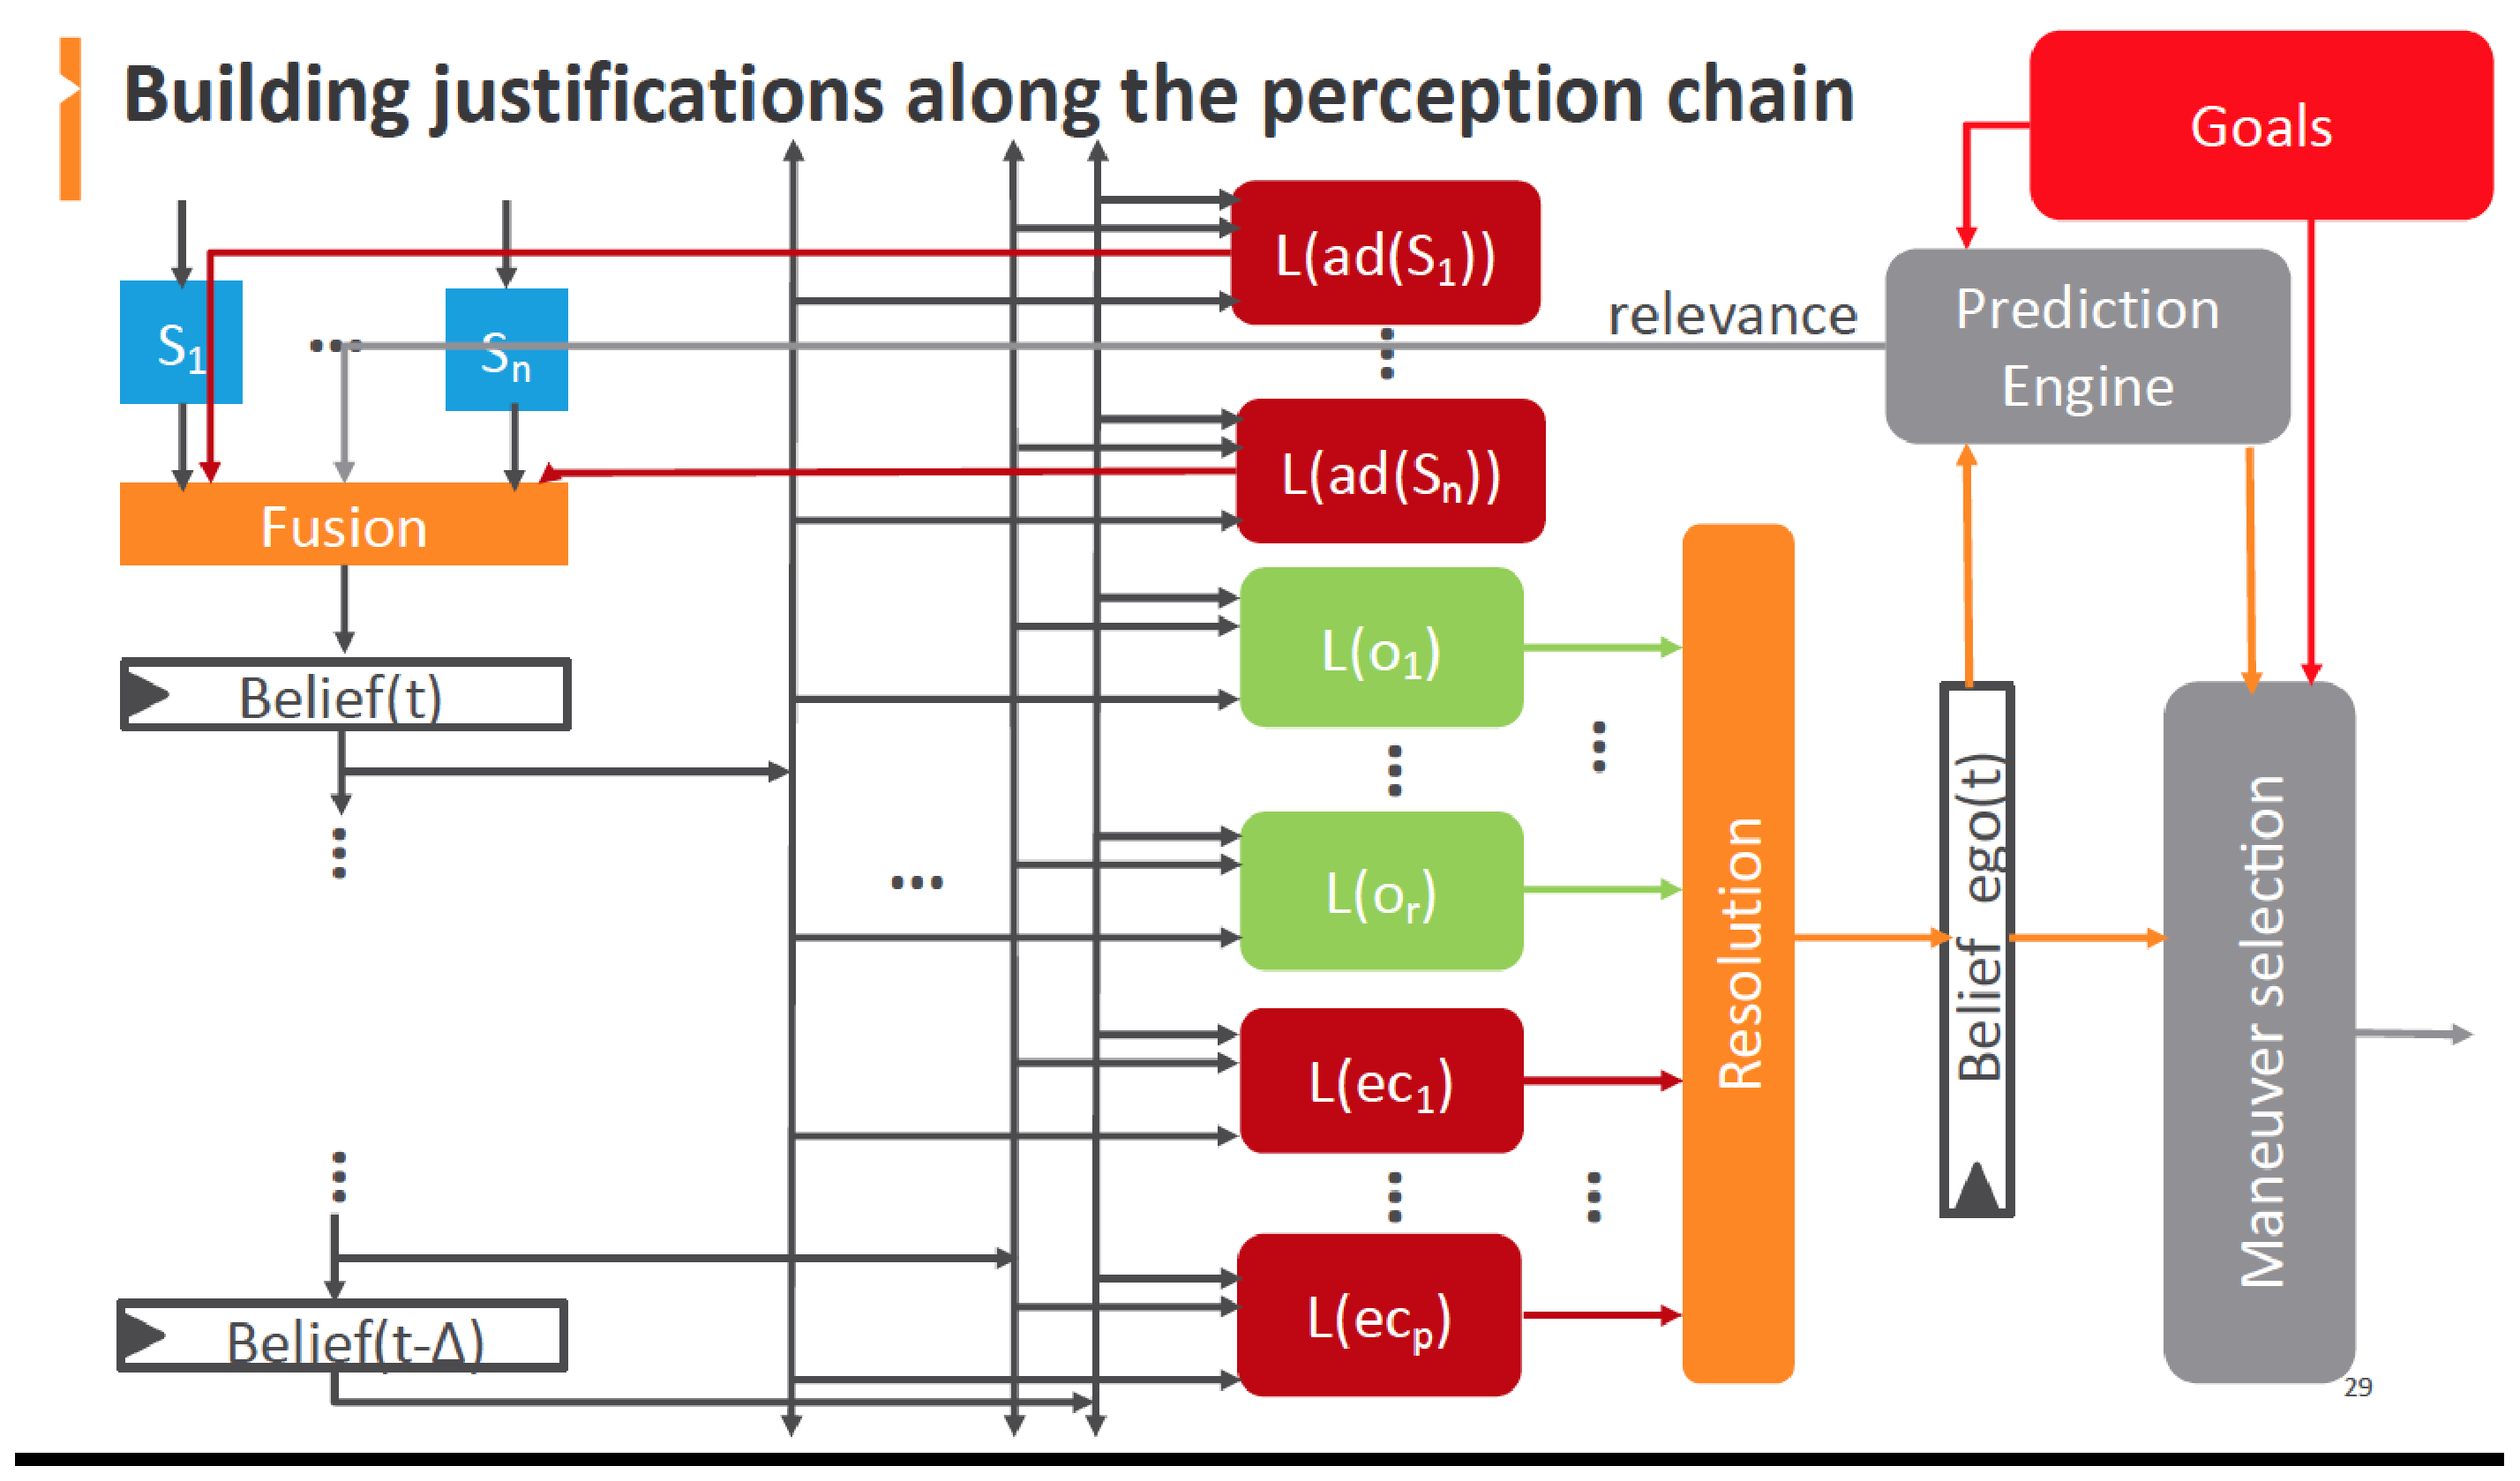
\includegraphics[width=\textwidth]{fig2.eps}
    \caption{Reference architecture}
    \label{fig:architecture}
\end{figure}
Figure \ref{fig:architecture} shows the proposed functional reference architecture of the perception chain, where belief(t) represents the labelled occupancy grid resulting from fusion of sensors s1 to sn, as discussed in Sect. \ref{subsec:quality}. We distinguish these from the complete reconstruction of the environment of the ego car, belief(ego), and assume that for each artifact  a in the ontology we have a dedicated learning component  L(a) for detecting both presence and absence of a in fields of the occupancy grid, see below. Note, that we assume that the prediction engine provides feedback about the relevance of fields in the occupancy grid, based on knowledge about the current beliefs of the ego car, and its current goals. Note also, that the learning components for identifying adverse sensor conditions are fed backwards into the sensor fusion unit. We propose the following measures to reduce the error of misperception:
\begin{enumerate}
\item To be able to exploit physical laws to optimize the prediction rate, we propose to maintain copies of such beliefs over some time window $\Delta$, and feed this into the classification network. This supports both object tracing as well as detection of misclassification in the resolution phase, since e.g. a pedestrian can not cross a four-lane street in one second.
\item We require for each learning component L(a) and each position in the electronic horizon to output both strength of beliefs for presence and for absence of a. We will only pass on classification votes of L(a) into beliefs of ego in the resolution process, if such strength values are separated by a safety margin determined in the validation phase of L(a), ensuring full separation for all test points.\todo{Letztlich muesste das doch bereits die Ontologie erledigen: Hier muesste doch ggf. sofort $\bot$ herauskommen.}
\item We use the ordering relation of the ontology to detect misclassifications in the resolution phase. E.g. identifying simultaneously a car and a pedestrian and the same location is impossible, unless both a car and a pedestrian where within reach to this location in the previous belief, taking into account the laws of physics capture in the respective behavioral models. Similarly, we detect inconsistencies in classification for ordered elements in the ontology, e.g. identifying a racing car by claiming that the same location does not contain a car.
\item We propose in-the-field learning for adverse conditions, by constantly comparing the individual sensors perception of the occupancy grid with the result from sensor fusion, including detection of inconsistencies. Under current regulation, such an on-line learning process must be done on a separate copy of the network and subjected to off-line verification and validation before activating it.
\end{enumerate}
$>>>>$ space permitting, I could still give an operational characterization of the resolution operator at this point: $>>>>$\\
\textcolor{blue}{This is non-trivial, because if will have to argue about the reach set, and needs to trace objects through time}

Section \ref{sec:proofrule} will show how quantify the risk of misperception, by incrementally working from the guarantees of type (3) for individual sensors, through sensor fusion, through the classification network, to the resolution stage, considering the above features for detecting inconsistencies.


%Werner with some help to be determined\\
%3 pages	concluded at page 7,5\\
%nur die Abweichungen zu diesem Bild die wir in den letzten beiden Runden besprochen haben
